\section{Context Free Grammar Stats}
\subsection{Introduction}
Fuzzing with context free grammars is done by making choices. Specifically, a
rule needs to be chosen at each non-terminal, each of which includes additional
terminal and/or non-terminal symbols. Eventually, after making many choices, a
point is reached in where there is no other non-terminal left to choose rules
from and one is left with a string of terminal symbols.

The ``quality`` of the generated output depends completely upon the choices
which are made. Therefore, it is critical to have some sort of way of making
``good`` choices: some way other than simply choosing a random rule from a
non-terminal. This is where statistics come in.

If Fuzzbuzz is able to take in various tables of statistics then it will
inherently be able to make informed choices. For example, a basic statistics
table might include production probabilities. That is to say, given some
non-terminal and its set of rules, what are the probabilities for each rule?
Given the following simple grammar, the table would provide $\mathbb{P}[B]$,
$\mathbb{P}[C]$, and $\mathbb{P}[D]$ where $\mathbb{P}[B] + \mathbb{P}[C] +
\mathbb{P}[D] = 1$.

\begin{center}
$A \rightarrow B$
\end{center}
\begin{center}
$\rightarrow C$
\end{center}
\begin{center}
$\rightarrow D$
\end{center}

This is certainly much better than making random choices, but it is still
rather basic. We now present a literature review of picking rules given a CFG.

\subsection{Literature Review}

Maurer\cite{Maurer1990} gives a wide range of ideas for choosing rules. In his
paper, he describes a simple calculator grammar and then focuses on various
ways he could use the grammar to test his calculator program. He gives various
ideas for picking rules, though he does not go in depth as to whether following
them produces better results. He mentions how one possibility is to avoid
choosing the same rule twice, or how perhaps rules should be chosen in a
particular order. Maurer, however, focuses a lot on user customization,
something which we do not. For example, Maurer suggests altering the
probabilities manually (which he refers to as weights). He reasons that by
doing so, one can generate tests which focus more in a particular area that is
believed to have bugs.

Maurer also suggests keeping track of the number of bugs encountered when a
particular rule is chosen, and then auto adjusting the probabilities to favor
those rules which detect the most bugs. We found this to be an interesting
approach.

Sirer and Bershad\cite{Bershad1999} describe their experience with using
production grammars in order to test software. Their paper does not exactly
propose ways of using statistics to pick rules, though it does suggest other
criteria you can use in order to come to a decision. The authors were working
primarily with the Java programing language, and as such some of their ideas
cater to Java specifics, though are nevertheless interesting enough to be
mentioned in this paper.

One approach which Sirer and Bershad discussed was imposing a limit on how many
times specific grammar rules can be exercised. This is especially useful in
languages like Java that have structural limits such as code length per
method. The authors describe another way in which this can turn out to be
useful: if one wants to ensure that the program doesn't ``terminate early``
(i.e. that it is of a minimum length) is to, for example, set a limit on your
start symbol to 5000 and then a probability of zero on the production $S
\rightarrow \lambda$. This will ``force`` a stop rather than ``naturally``
stopping.

In addition to using production limits, Sirer and Bershad also mention how
probabilities are of good use and emphasize the usefulness of separating
probabilities from the grammar. This is effectively what we do by having
Fuzzbuzz take a statistics table as a parameter which is distinct from the
actual grammar file.

Finally, Sirer and Bershad mention how in order to simplify future test
selection and analysis, for each test case produced they create what they call
a ``summary file`` which lists the name of the grammar rules that have rise to
the test case.

Though we did not find a paper which described conditional probabilities, we
did implement a routine in Gramstats which outputs conditional probabilities.
The conditional probabilities table describes what the probability of choosing a
specific rule is given what the previous N non-terminals were that led to our
current non-terminal. Our hypothesis was that knowing this information would
allow us to make better choices. For example, consider the following grammar:

\begin{center}
$S \rightarrow A$
\end{center}
\begin{center}
$\rightarrow A B$
\end{center}

\begin{center}
$A \rightarrow B C$
\end{center}
\begin{center}
$\rightarrow C$
\end{center}

\begin{center}
$B \rightarrow r C$
\end{center}
\begin{center}
$\rightarrow r$
\end{center}

\begin{center}
$C \rightarrow s B$
\end{center}
\begin{center}
$\rightarrow q$
\end{center}

where uppercase letters are non-terminal symbols and lowercase letters are
terminal symbols.


In this example, one could see how the probabilities for the rules $B
\rightarrow rC$ and $B \rightarrow r$ might differ depending on what the
previous non-ternminals were. For example, perhaps there is a much higher
probability of choosing $B \rightarrow r$ compared to $B \rightarrow rC$ if the
previous two non-terminals were $S$ and $A$ respectively. On the other hand, if
we arrive at $B$ though $A$ and $C$ respectively, then perhaps there is a
higher probability of choosing $B \rightarrow rC$ over $B \rightarrow r$.

Conditional probabilities allow us to keep more context than pure production
probabilities alone.

It is worth noting that the more you remember (i.e. the higher N is), the more
specific you become and thus the harder it is for Fuzzbuzz to actually be in
that state when generating. For example, taking an arbitrary grammar, if N=2,
then your ``memory`` could possibly be $F, R$ whereas if N=5, it could possibly
be $F, R, G, T, Q$. You can see how it is ``easier`` to land in a state where
your previous non-terminals are $F, R$ than $F, R, G, T, Q$. If while in some
iteration generating output the previous non-terminals are $F, R, G, X, Q$ then
$F, R$ passes but $F, R, G, T, Q$ does not.

\subsection{Results}

We ended up with two statistics tables to pass Fuzzbuzz as an argument to the
CFGStats engine: pure production probabilities and conditional probabilities.
By using the conditional probabilities we were able to produce far better
output. In our tests, when using production probabilities, Fuzzbuzz would
output programs which were much shorter than those using conditional
probabilities. For example, when using a simple calculator grammar,
using production probabilities would often result in output consisting of
single numbers, or a single addition/subtraction. When using conditional
probabilities, we often got long output with a mixture of matrices, vectors,
exponentiation and more.

Because of this, we focused all of our testing using conditional probabilities
rather than pure production probabilities alone.

We tested the CFGStats engine by comparing statistics from a corpus written by
a human (so, ``natural data'') to a corpus generated by Fuzzbuzz itself. This
second corpus is generated by running the Fuzzbuzz CFGStats engine 400 times and
each time feeding it into the Fuzzbuzz Mutation engine which produces Abstract
Syntax Trees for the output generated by CFGStats. Then, the sister tool
Gramstats can be used to analyze the ASTs produced by Fuzzbuzz Mutation.
Ideally, CFGStats's graphs and tables should be almost identical when comparing
the human input to the generated input as this would prove that our fuzzer is
producing realistic data.


\begin{figure*}
    \begin{center}
        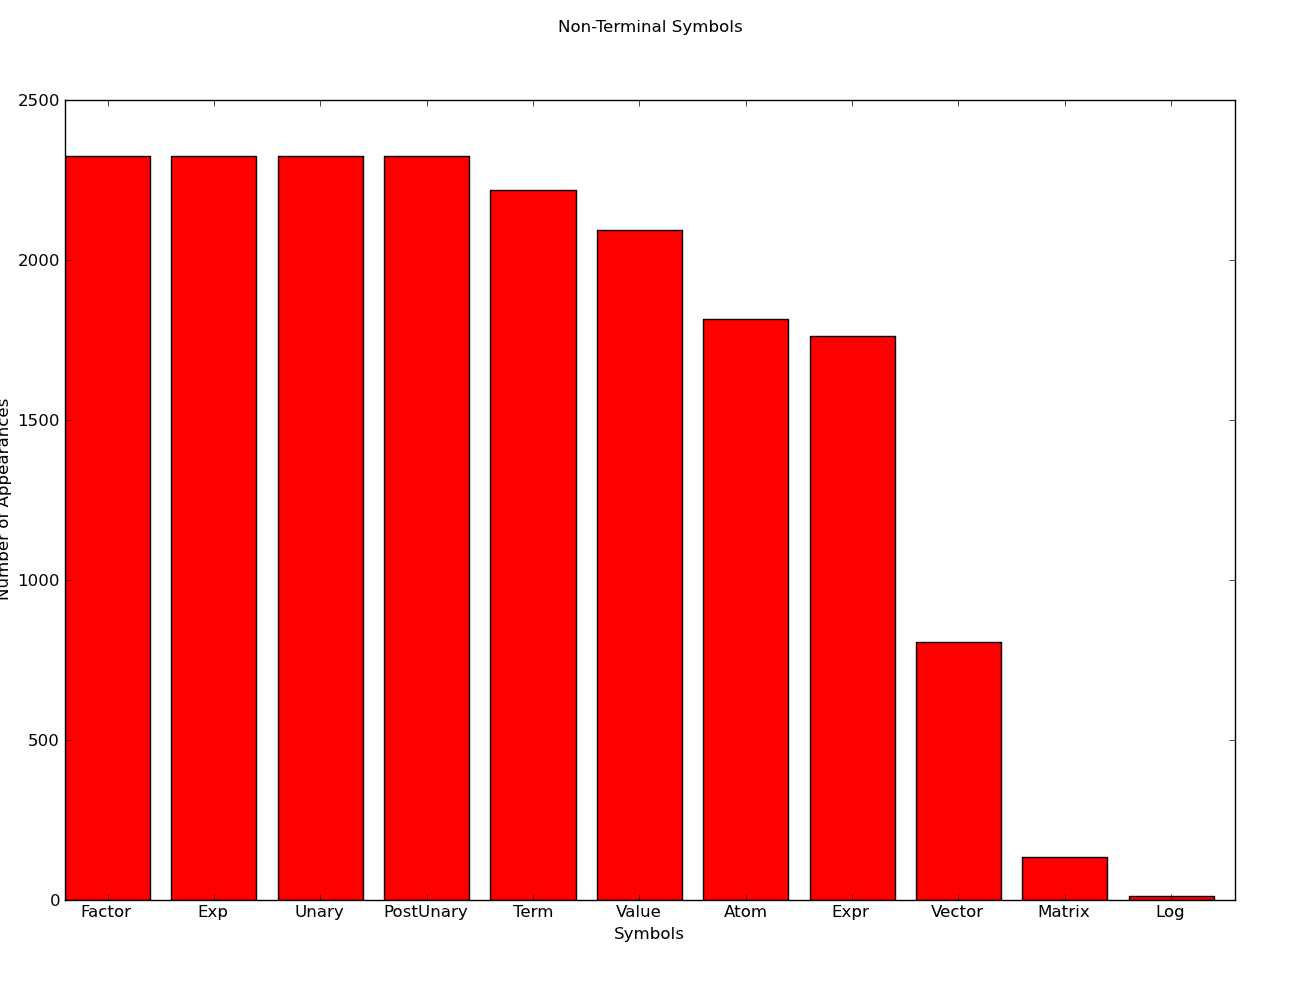
\includegraphics[scale=0.4]{figs/human/nonterm_histogram.png}
    \end{center}
        \caption{Average time spent calculating edit distance on a
                logarithmic scale. PQ-delim used a colon delimiter, PQ-explode
                used an explode delimiter, and PQ was run with the extended
                AST.}
    \label{times}
\end{figure*}
















